%----------------------------------------------------------------------------
\chapter{Background}
\label{sec:cfa}
%----------------------------------------------------------------------------


%----------------------------------------------------------------------------
\section{program representation}
\label{sec:program}
%---------------------------------------------------------------------------- 

A program most commonly is represented by a source code. Example: Euclid's algorithm in c

\begin{lstlisting}[language=C,breaklines=true]
int main(string args[])
{
	int arg1, arg2; //search for the highest common divisor of the 2 argument
	arg1 = args[0];
	arg2 = args[1];
	if(arg1>1000000 || arg1<=0 || arg2>1000000 || arg2<=0)
	{
		exit(1); //if the arguments are not supported we exit
	}
	for(arg1!=arg2)
	{ 
		if(arg1>arg2){
			arg1=arg1-arg2;
		}
		else{
			arg2=arg2-arg1;
		}
	}
	assertTrue(arg1==arg2);
	return arg1;	
}
\end{lstlisting}

There are many different type of code languages, making an abstract interpretation for all, would be hard and unnecessarily time-consuming. we need a common representation for programs on which we only need to make one abstract analyzer.

%----------------------------------------------------------------------------
\section{\cfa (CFA)}
\label{sec:cfaleiras}
%---------------------------------------------------------------------------- 
CFA can describe the programs as graphs, where edges are annotated with program statements. The Theta framework \hyperref[sec:ref]{[4]} provides a representation of a CFA formalism.

A CFA is a directed graph with
 
\begin{itemize}
	\item variables,
	\item locations, with dedicated initial, final and error locations,
	\item edges between locations, labeled with statements over the variables.
\end{itemize}

Statements can be:

\begin{enumerate}
	\item Assume: check if a condition is true for the variables
	\item Assign: assign a concrete value to a variable
	\item Havoc: assign a random value to a 
	\item Skip: no action
\end{enumerate}

The code in the \ref{sec:program} section translates to the CFA in figure \ref{fig:cfa}

\begin{figure} [!ht]
	\centering
	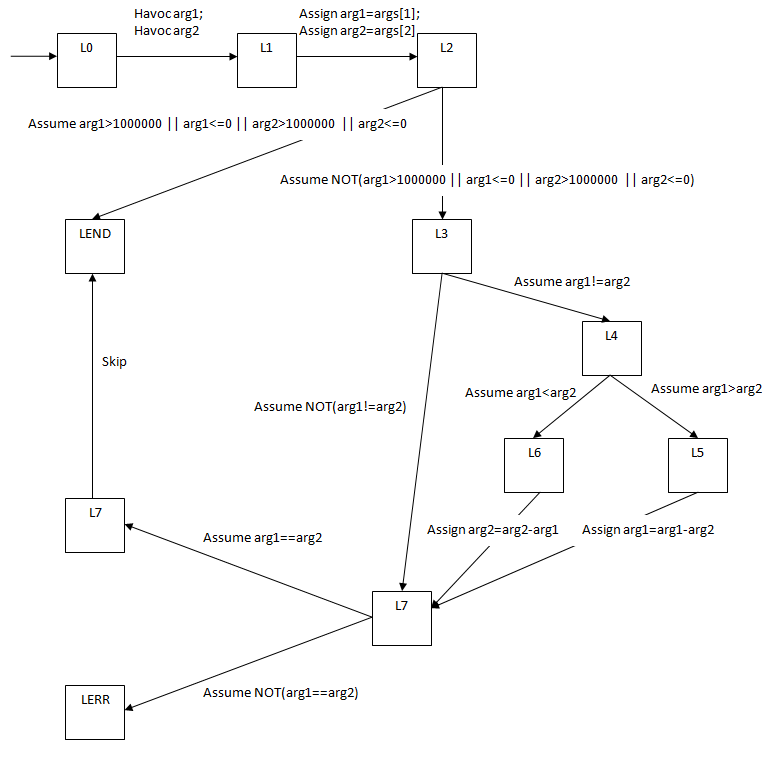
\includegraphics[width=170mm, keepaspectratio]{figures/cfa.png}
	\caption{\label{fig:cfa} CFA representation of Euclid's algorithm}
\end{figure}

Analysis is usually made for reachability of the error state. As seen in the example, assertions in the code can be used to create error states in the cfa. So in the end of the Euclid's algorithm if $arg1==arg2$ assertion fails we go to an error state. if there are more than one assertions in a code we can define one error state, and if the assertion fails we go to this error state.

So making sure that our code works properly now can be decided by the reachability of the error state. If we can prove it mathematically that the error state can not be reached than we proved that all of our assertions were satisfied, and therefore our program on the observed invariant is error free.


%----------------------------------------------------------------------------
\section{Motivation}
\label{sec:motivation}
%----------------------------------------------------------------------------
There are many formalisms for reachability analysis such as Bounded Modell Checking, which can provide a good counter example, a route to the error state. However the runtime -which depends on a good SMT solver- on really big cfa-s can be way too long. Also it can not prove that the error state is unreachable since it can only check bounded length of counter examples.

In order to make sure that there is no route to the error state we need to check all of them. Checking all the possible routes however can easily mean we have to examine infinite possibilities. For example the routes can differ, because of a variable's starting value -infinite possibilities for that- which already means it can have infinite different outcomes. To narrow down these possibilities abstraction can be really efficient. For example depending on our abstraction type we can make the similar routes into one group and instead of the infinite routes we will have a finite number of groups. One group contains those routes which are working in the same way on the abstraction, but it worked differently on the original.

The easiest example if we have a code:
\begin{lstlisting}[language=C,breaklines=true]
int main(string args[])
{
	int arg = args[0];
	if(arg<=0){
		//do something
	}
	if(arg>0){
		//do other things
	}	
}
\end{lstlisting}

$arg$ can have infinite possible values so the program should have infinite routes, however if we use interval abstraction we can set two different groups that are working the same way, and this two contains all the possible values. $GroupOne:arg=(-\infty;0); GroupTwo: arg=(1;\infty)$

%----------------------------------------------------------------------------
\section{Abstraction in general}
\label{sec:general}
%----------------------------------------------------------------------------

The goal of the abstraction is to make it possible to compute \emph{in reasonable time} that a certain error location is reachable or not. In theory there are three obstacles that make it impossible.

\begin{enumerate}
	\item There can be infinite amounts of location
	\item There can be a route (from the initial location), which is infinite (never reaches an end location)
	\item There can be infinite amount of different routes.
\end{enumerate}

Number 1 problem in cfa-s will not occur since locations are in between program statements and there can only be finite amount in one code.

Number 2 problem will be solved by fixpoints. See definition \ref{def:fixpoint}

Number 3 abstraction on the possible variables makes the similarly working routes the same, therefore narrowing the possibilities to a finite group of routes. See section \ref{sec:motivation}

%----------------------------------------------------------------------------
\section{Abstraction analysis algorithm for CFA}
\label{sec:cfaalgorithm}
%---------------------------------------------------------------------------- 
%TODO graphical representation of the algorithm

The goal of the abstraction interpretation algorithm as shown in figure \ref{fig:absanalyzer} is to state whether the error location is reachable or not. For this we need the CFA representation of the program and the abstraction type. More specifically a full library for that abstraction type, but we will expand on that later.

In the industrial world our goal is to prevent any erroneous behavior of our safty critical system. So detecting that an error exists is more important than to prove that the error not exists. Since the damage is much more costly if we fail in the first one. Imagine, if we say that there is no problem in our software that runs the subway system, but indeed there was, it can cause trains to collide which can cause serious -even life threatening- accidents. However, if we say that there is a possible error, the programmer can check, if that is really possible, and worse scenario is that he spent a lot of time examining the problem and found out that it is not possible, the damage is not that big.

\begin{figure} [!ht]
	\centering
	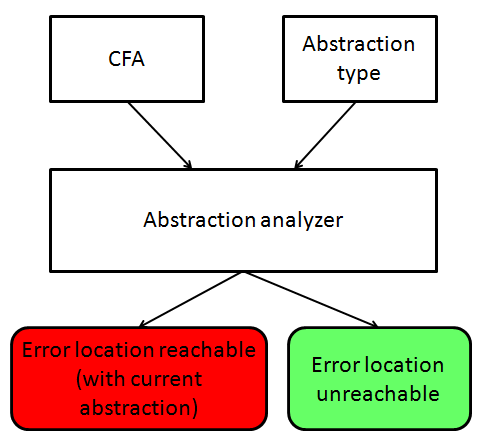
\includegraphics[width=100mm, keepaspectratio]{figures/abstractanalyzer.png}
	\caption{\label{fig:absanalyzer} Abstraction analysis model}
\end{figure}

The question is to find a valid route from the initial location to the error location. Valid means that every step of this route were possible. It depend on the variables that the location has. As we already discussed it is efficient to do some type of abstraction on these variables. In our work we will focus on interval abstraction, but there can be of course many other such as sign abstraction.

Abstraction interpretation on CFA-s means that we try to discover all the reachable locations starting from the initial location of course. We will put a label on every location that we have reached, and if no more label can be put -or changed- we reached a fixpoint (see definition \ref{def:fixpoint}).

The purpose of the label is not only to mark the reached location, but also is to be able to tell whether an out edge from the location can be possible or not. That of course depends on the variables in the program, so the label is some kind of representation of the possible variable values at the location that have been marked with it. In abstract interpretation this is of course some abstract form of the values. in sign abstraction it can be the possible signs of the variable in the location.

So one thing that an abstraction type should provide is a label for the variables, from which we can decide an assumption out edge is possible, and this label should be able to follow the changes of assign and havoc out edges. Now let us say that it is given.

So the first step is to put the initial label on the initial location. (let us say that an initial label is given for any abstraction type). Then let us say that the reached locations (marked with label) set is $ReachedLocations={initialLocation}$. The next step is to see if we reached an error location already. If we did we can stop, because an error location is reachable. Otherwise we do the next iteration.

In the next iteration we get all of the out edges of the $ReachdLocations$. And if the label allows it, than we put a new label onto the target location. There can be two different scenario. First the target location has no label yet,than this is a new location, we put the source location's label modified by the edge (assumption, assignment or havoc of course given by the abstraction type). Second the target location already has a label. In this case the change can widen or narrow the possibilities on that location. Narrowing it should not be possible though since if the values on this location already can exist it should still exist later. However widening can occur a lot of consecutive times for example in a cycle. To make it more reasonable we can use widening tactics.

We use widening tactic if a certain location's possible values widens. For example if a cycle grows a variable by one in every cycle finding the fixpoint can be time consuming. So the main idea is to widen the possible values more than we actually should and therefore find the limitation earlier. There can be more possible tactics, but it is important to make sure that in the end we only allow the possible values.

So the iteration ends if we can reach the error location, or if we found a fixpoint. If we found a fixpoint it means that the error location is unreachable. This is proven, if the abstraction label functions were implemented correctly, but it does not depend on which abstraction type was used. On the other hand if we reached the error location, we can only say that the error can be reached with the current abstraction. It is still possible that the error can not be reached, just we lost too many information during abstraction.

As we stated we need an abstraction type for the abstract interpretation. figure \ref{fig:abstype} shows the summary of what we except from an abstraction type to be able to do.

\begin{itemize}
	\item initial label: be able to mark an initial location (here every values should be possible)
	\item isValid: beang able to tell if after the assumption out edge the result can be valid (there are still possible values)
	\item addLabel: being able to change a given location's label with assignment, assumption or havoc out edge
	\item wideningtactic: The widening tactic should be specified (it depends on the label type)
	\item partitioningtactic: This applies the assignment, assumption or havoc statements to the label
\end{itemize}

Partitioning has not been mentioned, because in our work we did not implement any partitioning tactics. However our library gives the possibility to implement one. We will show some possible partitioning for interval abstraction.

\begin{definition}{fixpoint}
	\label{def:fixpoint}
	A fixpoint is when no further refinement can be made on the discovered reachable locations and no more location is reachable.
	In CFA this will mean that none of the outedges in any of the reached location can reach a new location nor can change the label of the reached locations.
\end{definition}

\begin{figure} [!ht]
	\centering
	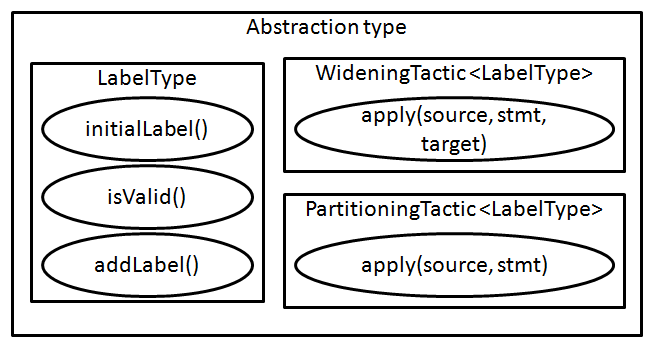
\includegraphics[width=150mm, keepaspectratio]{figures/abstractiontype.png}
	\caption{\label{fig:abstype} The structure of an Abstraction type}
\end{figure}








